\justifying
Στην παρούσα εργασία, τα σήματα που θα διαχωριστούν θα αναφέρονται σε βιολογικές εφαρμογές και αποκαλούνται \emph{βιοσήματα}. Συγκεκριμένα, θα γίνει ανάλυση σημάτων με βάση το δυναμικό δράσης στην κυτταρική μεμβράνη, χρησιμοποιώντας για την μέτρηση του διακυτταρικά ηλεκτρόδια. Τέλος, τα σήματα αφορούν την λειτουργία της καρδιάς και για την αναπαράστασή τους γίνεται χρήση ηλεκτροκαρδιογραφημάτων. 
\section{Ανατομία της Καρδιάς}
\justifying
Η καρδία \cite{heart:23} \cite{heart:26} είναι ένα κοίλο μυώδες όργανο σε μέγεθος περίπου όσο μια γροθιά. Για τους άνδρες έχει βάρος 250-350 γραμμάρια, ενώ στις γυναίκες είναι 240-280 γραμμάρια. Βρίσκεται ανάμεσα στους δυο πνεύμονες πίσω από το στέρνο. Η θέση της εξωτερικά αντιστοιχεί από τον 3ο έως τον 6ο πλευρικό χόνδρο. Τέλος, επικάθεται στο διάφραγμα και όταν συστέλλεται, κινείται προς τα εμπρός και αριστερά.
\\[0.3 \baselineskip]
Η καρδιά βρίσκεται μέσα σε ένα λεπτό σάκο ινώδους ιστού που ονομάζεται \emph{περικάρδιο} και έχει 3 στρώματα ιστού: το επικάρδιο, το μυοκάρδιο και το ενδοκάρδιο. Το \emph{επικάρδιο} είναι μια λεπτή μεμβράνη που καλύπτει την επιφάνεια της καρδιάς. Κάτω από το επικάρδιο, βρίσκεται ένα παχύ στρώμα μυός που ονομάζεται \emph{μυοκάρδιο}. Τέλος, το εσωτερικό μέλος της καρδιάς καλύπτεται από μια μεμβράνη που ονομάζεται \emph{ενδοκάρδιο} και καλύπτει το εσωτερικό των κοιλοτήτων της καρδιάς, τις βαλβίδες και τους μυς στις κοιλότητες που συνδέονται με τις βαλβίδες.
\\[0.3 \baselineskip]
Η καρδιά αποτελείται από 4 κοιλότητες ( Σχήμα \ref{fig:2.1} ). Οι δύο είναι πιο μεγάλες και με παχιά τοιχώματα που ονομάζονται \emph{κοιλίες} και οι άλλες δύο είναι μικρότερες και με λεπτότερα τοιχώματα που ονομάζονται \emph{κόλποι}. Οι κόλποι χωρίζονται με το \emph{μεσοκολπικό διάφραγμα} ενώ οι κοιλίες με το \emph{μεσοκοιλιακό διάφραγμα}. Το μεσοκοιλιακό διάφραγμα εμποδίζει το αίμα να περάσει από την μία πλευρά της καρδιάς στην άλλη, καθώς η δεξιά πλευρά γεμίζει πάντοτε από φλεβικό αίμα ενώ η αριστερή από αρτηριακό.
\\[0.3 \baselineskip]
Όσο αφορά την λειτουργία της καρδιάς, ο δεξιός κόλπος δέχεται το αίμα από όλα τα μέρη του σώματος μέσω των μεγάλων φλεβών, τα προωθεί στην δεξιά κοιλία και από εκεί στους πνεύμονες με στόχο την οξυγόνωση τους. Στην συνέχεια, το αίμα προωθείται από τους πνεύμονες στον αριστερό κόλπο και στην αριστερή κοιλία. Τέλος, με την συστολή της καρδιάς, το οξυγωνομένο αίμα προωθείται από την αριστερή κοιλία στο υπόλοιπο σώμα, μέσω της αορτής και των μεγάλων αρτηριών.
\begin{figure}[H]
    \centering
    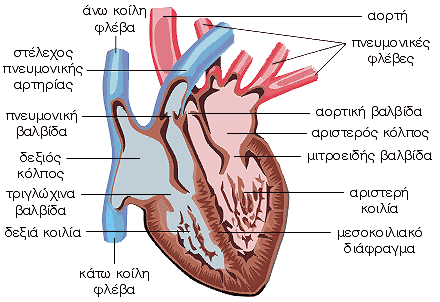
\includegraphics[width=0.8\textwidth]{misc/heart-anatomy.png}
    \caption{Εσωτερική όψη καρδιάς}
    \label{fig:2.1}
\end{figure}
\noindent Η καρδιά συντονίζεται από εσωτερικούς φυσικούς βηματοδότες, οι οποίοι είναι ο \emph{φλεβόκομβος}, που βρίσκεται στο τοίχωμα του δεξιού κόλπου και ο \emph{κολποκοιλιακός κόμβος} που βρίσκεται στο σημείο επαφής του μεσοκολπικού με το μεσοκοιλιακό διάφραγμα.
\\[0.5 \baselineskip]
Η καρδιά, επιπλέον, διαθέτει 4 \emph{βαλβίδες} που χρησιμεύουν στο να επιτρέπουν την δίοδο του αίματος προς μία μόνο κατεύθυνση και να εμποδίζουν την παλινδρόμηση του κατά τη διάρκεια της καρδιακής συστολής. Οι βαλβίδες αποτελούνται από μικρά αλλά ισχυρά μέρη, τις γλωχίνες, και είναι υπεύθυνες για υποχρεωτική κυκλοφορία του αίματος προς μία μοναδική κατεύθυνση.
\\
Αυτές οι βαλβίδες είναι:
\begin{itemize}
    \item η \emph{τριγλώχινη} μεταξύ δεξιού κόλπου και δεξιάς κοιλίας.
    \item η \emph{πνευμονική} μεταξύ δεξιάς κοιλίας και πνευμονικής αρτηρίας.
    \item η \emph{μιτροειδής} μεταξύ αριστερού κόλπου και αριστερής κοιλίας 
    \item η \emph{αορτική} μεταξύ αριστερής κοιλίας και αoρτής.
\end{itemize}
όπως φαίνονται στο σχήμα \ref{fig:2.2}.
\\ [0.5 \baselineskip]
Το περικάρδιο εμποδίζει την σύμπτωση των βαλβίδων, καθώς αποτελεί σημείο πρόσφυσης μεταξύ του μυοκαρδίου και των γλωχίνων των βαλβίδων, ενώ ταυτόχρονα βοηθά στον διαχωρισμό της σύσπασης κόλπων και κοιλιών, δρώντας ως μονωτής του σήματος σύσπασης. 
\begin{figure}[H]
    \centering
    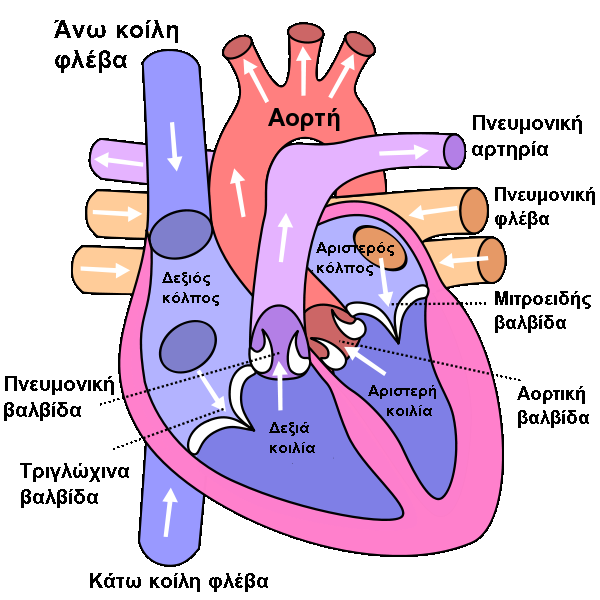
\includegraphics[width=0.7\textwidth]{misc/valves_of_heart.png}
    \caption{Κύρια μέρη της καρδιάς}
    \label{fig:2.2}
\end{figure}
\noindent Τέλος, για την αιμάτωση της, η καρδιά έχει δύο αγγεία, την αριστερή και την δεξιά \emph{στεφανιαία αρτηρία} που βρίσκονται στο αρχικό μέρος της αορτής. Ο βασικός τους ρόλος είναι να παρέχουν οξυγόνο και γενικότερα θρεπτικές ουσίες στα κύτταρα του μυοκάρδιου.
\section{Ηλεκτρική Φυσιολογία Καρδιάς}
\justifying
Ο καρδιακός μυς αποτελείται από κύτταρα που ονομάζονται \emph{καρδιακές μυϊκές ίνες}. Οι μεμβράνες των γειτονικών κυττάρων συνδέονται μεταξύ τους σε σειρά αλλά και πλάγια, δημιουργώντας ένα ενιαίο μόρφωμα. επιτρέποντας έτσι την ελεύθερη διάχυση των ιόντων. Έτσι, ο ερεθισμός και μίας μόνο μυοκαρδιακής ίνας οδηγεί σε εξάπλωση του δυναμικού δράσης σε ολόκληρη την μυϊκή μάζα.
\\[0.5 \baselineskip]
Όπως όλα τα κύτταρα του σώματος, έτσι και τα καρδιακά κύτταρα, έχουν ένα ηλεκτρικό δυναμικό στην κυτταρική τους μεμβράνη. Τόσο στον εξωκυττάριο όσο και στον ενδοκυττάριο χώρο υπάρχουν αρνητικά και θετικά φορτία (ιόντα) ίσα μεταξύ τους. Όμως, μέσα από την κυτταρική μεμβράνη υπάρχει περίσσεια αρνητικά φορτισμένων ιόντων, ενώ έξω από αυτή συγκεντρώνονται σε ίση ποσότητα θετικά φορτισμένα ιόντα. Το αποτέλεσμα είναι η \emph{πόλωση}, δηλαδή η διαφορά δυναμικού μεταξύ του εσωτερικού και του εξωτερικού της κυτταρικής μεμβράνης. Το δυναμικό αυτό ονομάζεται \emph{δυναμικό ηρεμίας} και έχει τιμή ίση με \en -90 mV.\gr
\\[2 \baselineskip]
Επιπλέον, τα καρδιακά κύτταρα είναι ικανά να μεταβάλλουν το δυναμικό της κυτταρικής τους μεμβράνης, έτσι ώστε να αναπτύξουν ένα ηλεκτρικό δυναμικό που διαδίδεται κατά μήκος της μυϊκής ίνας όταν διεγείρεται επαρκώς. Το δυναμικό αυτό είναι γνωστό ως \emph{δυναμικό δράσης}.
\\[0.5 \baselineskip]
Η καρδιά περιλαμβάνει δύο δυναμικά δράσης, ένα στο κολπικό μυοκάρδιο και ένα στο κοιλιακό μυοκάρδιο. Στο κοιλιακό μυοκάρδιο, το δυναμικό παράγεται από τα ρεύματα εκπόλωσης των γειτονικών κυττάρων και υπολογίζεται στα 105 \en mV, \gr αυξάνοντας το δυναμικό από τα -90 \en mV \gr στα περίπου 20 \en mV. \gr Μετά από το αρχικό έπαρμα, η μεμβράνη μένει σε κατάσταση εκπόλωσης για 0.15 δευτερόλεπτα στο κολπικό μυοκάρδιο έως και 0.3 δευτερόλεπτα στο κοιλιακό μυοκάρδιο, εμφανίζοντας ένα χαρακτηριστικό \en "plateau", \gr στο τέλος του οποίου ακολουθεί απότομη επαναπόλωση.
\\[0.5 \baselineskip]
Σε φυσιολογικές συνθήκες, η μυϊκή ίνα βρίσκεται σε κατάσταση ηρεμίας ή πόλωσης. Εάν διεγερθεί το ένα άκρο της με κάποιο ερέθισμα τότε ξεκινά αυτόματα η διαδικασία της εκπόλωσης και το ερέθισμα μεταφέρεται από το ένα άκρο της στο άλλο. Έπειτα ξεκινά απότομα το κύμα επαναπόλωσης που είναι ακριβώς αντίθετο με το κύμα εκπόλωσης.
\\[0.5 \baselineskip]
\begin{figure}[H]
    \centering
    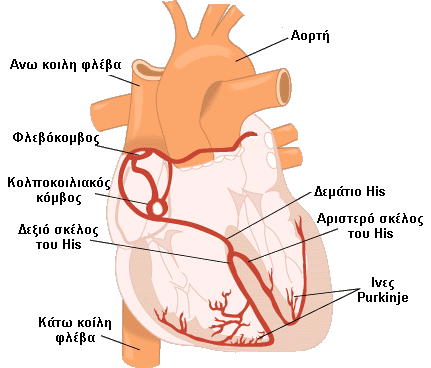
\includegraphics[width=0.7\textwidth]{misc/stimulus.png}
    \caption{Το ερεθισματαγωγό σύστημα της καρδιάς}
    \label{fig:2.3}
\end{figure}
Το ερεθισματωγό σύστημα της καρδίας (Σχήμα \ref{fig:2.3}) αποτελείται από τα εξής μέρη:
\begin{itemize}
    \item τον \emph{φλεβοκολπικό} και \emph{κολποκοιλιακό κόμβο}
    \item το κολποκοιλιακό \emph{δεμάτιο \en Hiss \gr} που χωρίζεται σε δεξί και αριστερό σκέλος
    \item τις \emph{ίνες του \en Purkinje \gr}
    \item τον \emph{φλεβόκομβο}
\end{itemize}
Ο φλεβόκομβος παράγει το πρώτο ηλεκτρικό δυναμικό, το οποίο ξεκινά αλυσιδωτή ηλεκτρική αντίδραση για την μετάδοση του ερεθίσματος σε όλο το τοίχωμα των κόλπων με αποτέλεσμα την σύσπαση τους. Η μετάδοση του ερεθίσματος στους κόλπους εξαπλώνεται σε 0.1 δευτερόλεπτα. Κατόπιν, περνά τον κολποκοιλιακό κόμβο και διαχέεται με μικρή καθυστέρηση στο δεμάτιο του \en Hiss \gr και ύστερα στις κοιλίες μέσω του δεξιού και αριστερού σκέλους του δεματίου, δημιουργώντας τους συστολή. Οι τελικές απολήξεις των στελεχών είναι οι ίνες του \en Purkinje, \gr οι οποίες προχωρούν κάθετα από το ενδοκάρδιο στο επικάρδιο.
\\[0.5 \baselineskip]
Η περίοδος από το τέλος μιας καρδιακής συστολής έως το τέλος της επόμενης ονομάζεται \emph{καρδιακός κύκλος}. Κάθε κύκλος ξεκινά με την αυτόματη παραγωγή ενός δυναμικού δράσης στον φλεβόκομβο και ολοκληρώνεται μετά το πέρας των 5 ακόλουθων φάσεων:
\begin{enumerate}
    \item την παθητική πλήρωση της καρδίας από αίμα
    \item την συστολή των κόλπων
    \item την διέγερση και ισομετρική συστολή 
    \item την εξώθηση του αίματος από την καρδιά
    \item την ισομετρική χάλαση
\end{enumerate}
\section{Ηλεκτροκαρδιογράφημα}
\justifying
Το \emph{ηλεκτροκαρδιογράφημα} ή \en \emph{ECG} \gr\cite{heart:26} είναι μία γραφική αναπαράσταση της εκπόλωσης και της επαναπόλωσης της καρδιάς, που καταγράφεται ως το δυναμικό που προκαλούν οι παραπάνω λειτουργίες και το οποίο διαδίδεται στην επιφάνεια του δέρματος.
\\[0.5 \baselineskip]
Ένα φυσιολογικό ηλεκτροκαρδιογράφημα φαίνεται στο σχήμα \ref{fig:2.4} και αποτελείτε από τα ακόλουθα διαστήματα και επάρματα:
\begin{figure}[H]
    \centering
    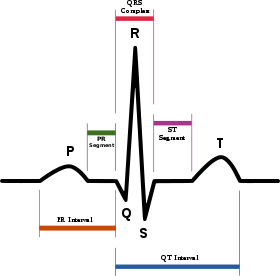
\includegraphics[width=0.7\textwidth]{misc/ECG.png}
    \caption{Χαρακτηριστικά μεγέθη ηλεκτροκαρδιογραφήματος}
    \label{fig:2.4}
\end{figure}
\begin{itemize}
    \item το \textbf{έπαρμα \en P\gr} που αντιστοιχεί στην κολπική εκπόλωση και έχει διάρκεια μικρότερη των 0.12 δευτερολέπτων. Ενίοτε εμφανίζεται θετικό ενώ άλλες φορές αρνητικό.
    \item το \textbf{διάστημα \en PR\gr} που αντιστοιχεί στο χρονικό διάστημα από την εκπόλωση των κόλπων έως την εκπόλωση των κοιλιών και για φυσιολογικά άτομα έχει διάρκεια από 0.12 έως 0.2 δευτερόλεπτα.
    \item το \textbf{σύμπλεγμα \en QRS\gr} το οποίο αντιστοιχεί στον ερεθισμό και στην εκπόλωση των κοιλιών και για φυσιολογικά άτομα έχει διάρκεια μικρότερη ή ίση των 0.10 δευτερολέπτων.
    \item το \textbf{διάστημα \en ST\gr} και το \textbf{έπαρμα \en T\gr} που αντιστοιχούν στην επαναπόλωση των κοιλιών. 
    
\end{itemize}
